\subsection{Giới thiệu}
Trong thuật toán K-means clustering, chúng ta không biết nhãn (label) của từng điểm dữ liệu. 
Mục đích là làm thể nào để phân dữ liệu thành các cụm (cluster) khác nhau sao cho dữ liệu trong cùng một cụm có tính chất giống nhau.
\par
\textbf{Ví dụ}: Một công ty muốn tạo ra những chính sách ưu đãi cho những nhóm khách hàng khác nhau dựa trên sự tương tác giữa mỗi khách hàng với công ty đó (số năm là khách hàng; số tiền khách hàng đã chi trả cho công ty; độ tuổi; giới tính; thành phố; nghề nghiệp; …). 
Giả sử công ty đó có rất nhiều dữ liệu của rất nhiều khách hàng nhưng chưa có cách nào chia toàn bộ khách hàng đó thành một số nhóm/cụm khác nhau. 
Nếu một người biết Machine Learning được đặt câu hỏi này, phương pháp đầu tiên ta nghĩ đến sẽ là K-means Clustering. 
Sau khi đã phân ra được từng nhóm, nhân viên công ty đó có thể lựa chọn ra một vài khách hàng trong mỗi nhóm để quyết định xem mỗi nhóm tương ứng với nhóm khách hàng nào. 
Phần việc cuối cùng này cần sự can thiệp của con người, nhưng lượng công việc đã được rút gọn đi rất nhiều.
\par
Ý tưởng đơn giản nhất về cluster (cụm) là tập hợp các điểm ở gần nhau trong một không gian nào đó (không gian này có thể có rất nhiều chiều trong trường hợp thông tin về một điểm dữ liệu là rất lớn). 
Hình bên dưới là một ví dụ về 3 cụm dữ liệu.
\begin{figure}[!htbp]
    \centering
    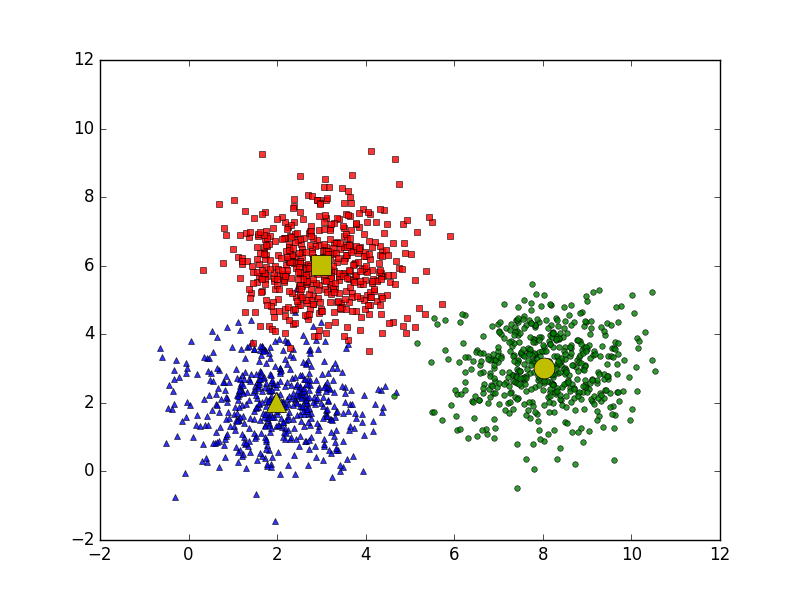
\includegraphics[scale=0.5]{kmeans}
    \caption{Bài toán với 3 clusters.}
    \label{fig:x cubed graph}
\end{figure}
\FloatBarrier
Giả sử mỗi cluster có một điểm đại diện (center) màu vàng. Và những điểm xung quanh mỗi center thuộc vào cùng nhóm với center đó. Một cách đơn giản nhất, xét một điểm bất kỳ, ta xét xem điểm đó gần với center nào nhất thì nó thuộc về cùng nhóm với center đó. Tới đây, chúng ta có một bài toán thú vị: \textit{Trên một vùng biển hình vuông lớn có ba đảo hình vuông, tam giác, và tròn màu vàng như hình trên. Một điểm trên biển được gọi là thuộc lãnh hải của một đảo nếu nó nằm gần đảo này hơn so với hai đảo kia . Hãy xác định ranh giới lãnh hải của các đảo}
\subsection{Phân tích chi tiết}
Đầu tiên là chuẩn bị dữ liệu cần phân cụm. Tiếp theo quyết định số lượng cụm (cluster) cần phân chia. Ở ví dụ này thử chọn số cluster là 3. Ở đây data được thể hiện dưới dạng các điểm cho dễ quan sát. Cự ly của các dữ liệu được hiểu là độ dài đoạn thẳng nối giữa 2 điểm với nhau.
\begin{figure}[!htbp]
    \centering
    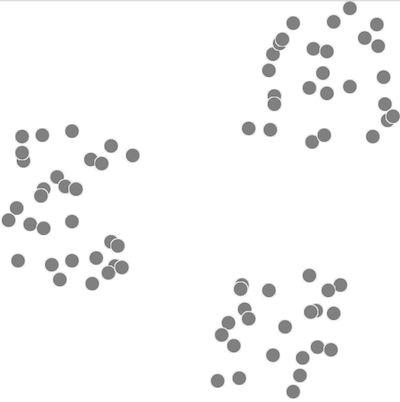
\includegraphics[scale=0.5]{kmeans_detail1}
    \caption{Cụm ban đầu.}
    \label{fig:x cubed graph}
\end{figure}
\FloatBarrier
\textbf{Bước 2}
\par
Chọn ngẫu nhiên 3 điểm làm điểm trung tâm của cluster.
\begin{figure}[!htbp]
    \centering
    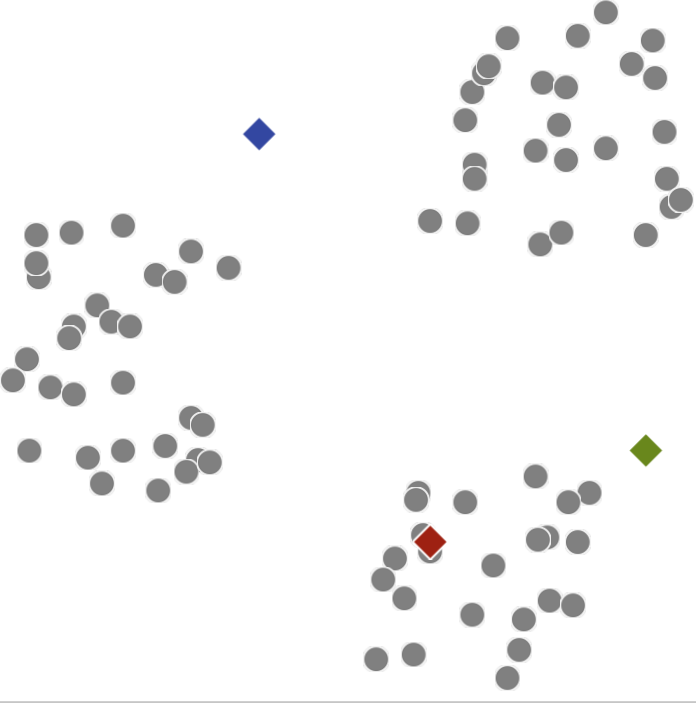
\includegraphics[scale=0.5]{kmeans_detail2}
    \caption{Chọn ngẫu nhiên trung điểm.}
    \label{fig:x cubed graph}
\end{figure}
\FloatBarrier
\textbf{Bước 3}
\par
Với các điểm dữ liệu không được chọn là điểm trung tâm thì tính toán khoảng cách từ chính điểm đó đến các cluster và quyết định cluster nào gần với mình nhất.
\begin{figure}[!htbp]
    \centering
    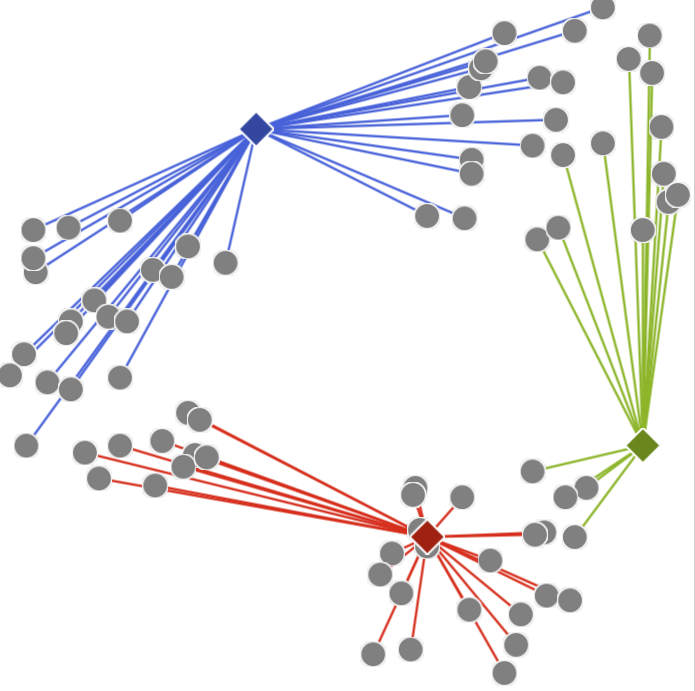
\includegraphics[scale=0.5]{kmeans_detail3}
    \caption{Tính toán khoảng cách tới điểm.}
    \label{fig:x cubed graph}
\end{figure}
\FloatBarrier
\textbf{Bước 4}
\par
Từ bước tính toán trên, tiến hành phân loại các điểm về các cluster đã quyết định(cluster gần nó nhất). Vậy là đã phân ra được 3 cụm.
\begin{figure}[!htbp]
    \centering
    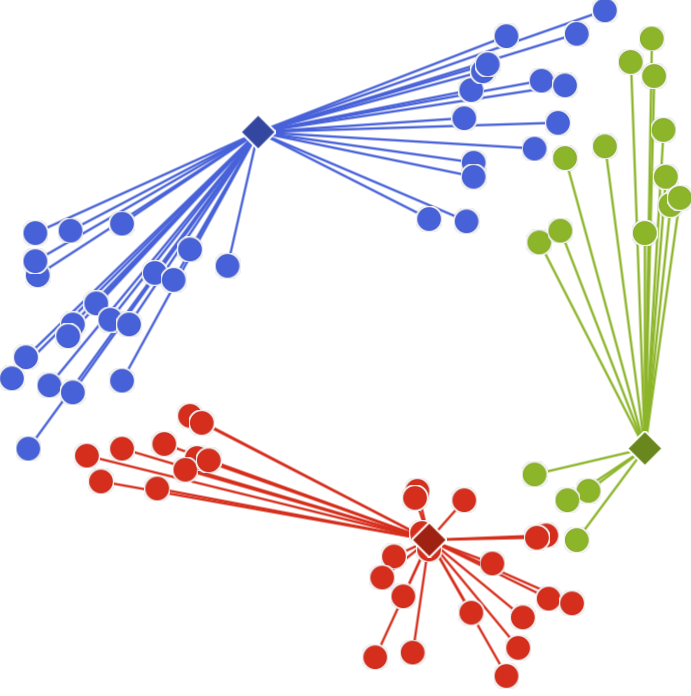
\includegraphics[scale=0.5]{kmeans_detail4}
    \caption{Phân thành 3 clusters.}
    \label{fig:x cubed graph}
\end{figure}
\FloatBarrier
\textbf{Bước 5}
\par
Bước trên chúng ta đã thu được 3 cụm, bây giờ tiến hành tính trọng tâm của các điểm dữ liệu của từng cụm. Sau đó di chuyển điểm trung tâm của cụm sang vị trí vừa tính được.
\begin{figure}[!htbp]
    \centering
    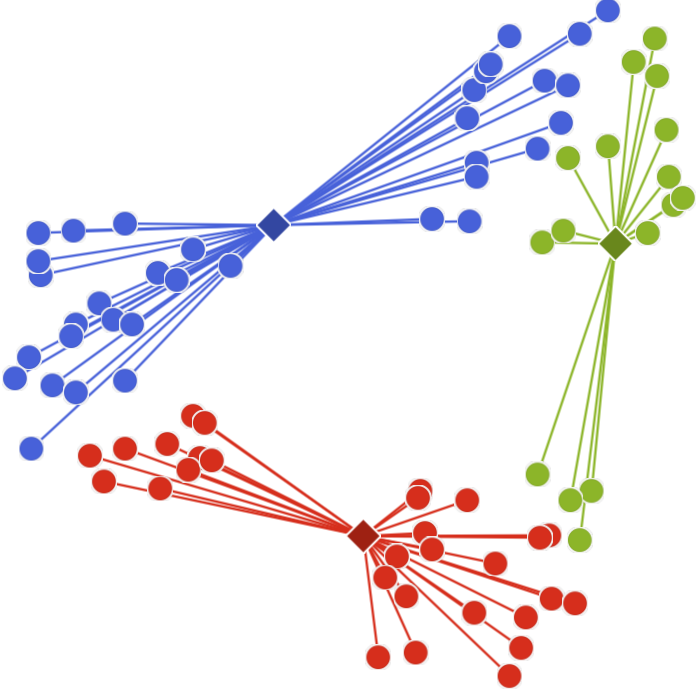
\includegraphics[scale=0.5]{kmeans_detail5}
    \caption{Tính trọng điểm.}
    \label{fig:x cubed graph}
\end{figure}
\FloatBarrier
Vị trí mà 3 điểm trung tâm của cluster vừa di chuyển đến được hiểu ngắn gọn chính là điểm trung tâm đang di chuyển đến vị trí chính xác hơn.
\newline
\textbf{Bước 6}
\par
Một lần nữa tiến hành bước 3, tính toán lại khoảng các các điểm đến các điểm trung tâm. Sau đó phân loại lại các điểm dữ liệu về các cụm.
\begin{figure}[!htbp]
    \centering
    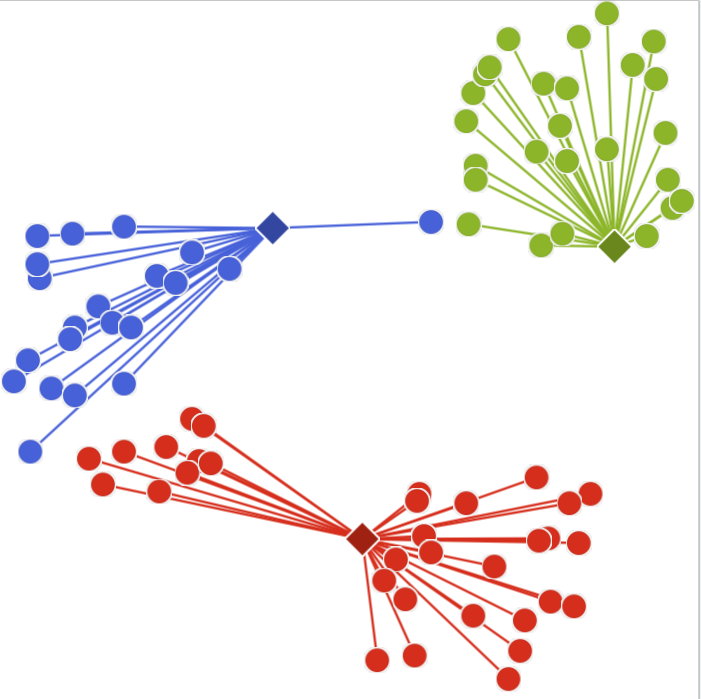
\includegraphics[scale=0.5]{kmeans_detail6}
    \caption{Tính toán lại khoảng cách.}
    \label{fig:x cubed graph}
\end{figure}
\FloatBarrier
\textbf{Bước 7}
\par
Sau đó lặp lại quá trình di chuyển cluster trung tâm và phân loại lại các điểm về các cụm gần nhất.
Quá trình này sẽ dừng khi sau khi dữ liệu sau khi phân cụm lại không thay đổi gì so với lần trước.
\begin{figure}[!htbp]
    \centering
    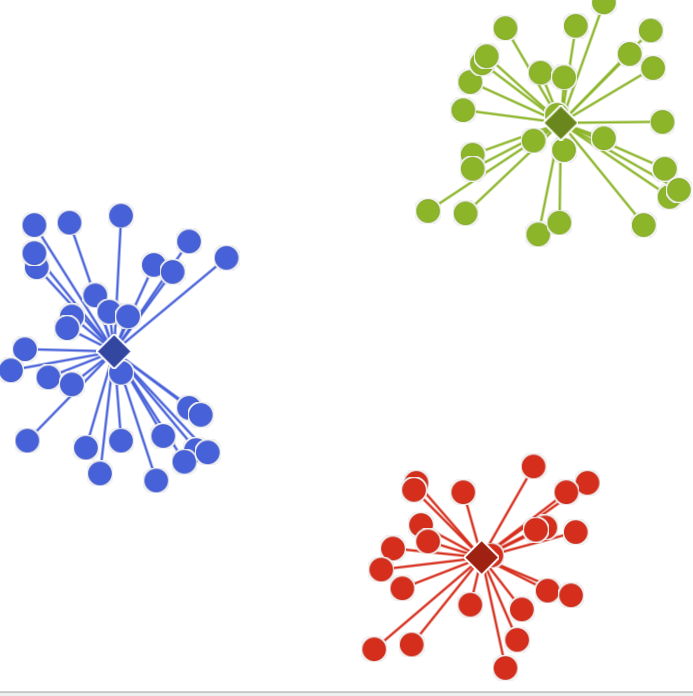
\includegraphics[scale=0.5]{kmeans_detail7}
    \caption{Kết quả.}
    \label{fig:x cubed graph}
\end{figure}
\FloatBarrier
\subsection{Lưu ý}
Trước khi sử dụng phương pháp này, chúng ta phải quyết định trước số lượng cluster, tuy nhiên trong quá trình tính toán số lượng cluster có thể khác với số lượng cluster mình dự đoán nên kết quả sẽ không chính xác.
\par
Vì vậy để giải quyết vấn đề này, để có thể chọn ra số lượng cluster thích hợp thì cần phải phân tích dữ liệu cẩn thận, chạy thử k-means với nhiều biến số số lượng cluster.
\par
Cùng ví dụ trên nếu thay số lượng cluster thành 2, kết quả phân loại sẽ thành ra như sau:
\begin{figure}[!htbp]
    \centering
    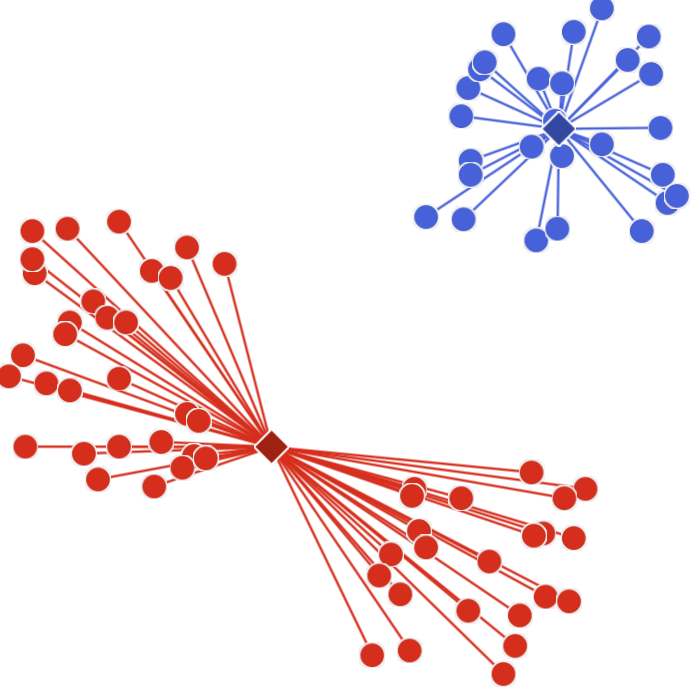
\includegraphics[scale=0.5]{kmeans_2_clusters}
    \caption{Khi chia thành 2 cụm.}
    \label{fig:x cubed graph}
\end{figure}
\FloatBarrier